\documentclass{article}
\usepackage[utf8]{inputenc}

\usepackage{amsfonts}
\usepackage{amssymb}
\usepackage{amsmath}
\usepackage{amsthm}
\usepackage{enumitem}

\usepackage{bbold}
\usepackage{bm}
\usepackage{graphicx}
\usepackage{color}
\usepackage{hyperref}
\usepackage[margin=2.5cm]{geometry}

\usepackage{float}

\newcommand\round[1]{\left[#1\right]}

\begin{document}

% ==============================================================================

\title{\Large{INFO8006: Project 3 - Report}}
\vspace{1cm}
\author{\small{\bf Maxime Goffart - s180521} \\ \small{\bf Olivier Joris - s182113}}

\maketitle

% ==============================================================================

\section{Bayes filter}

\begin{enumerate}[label=\alph*.,leftmargin=*]
    \item The observable evidence variables at time \textit{t} are defined in
    this way for the ghost \textit{i} : \\
    
    $NoisyDistance(i) = 
    ManhattanDistance(ghost(i), Pacman) + Binom(n, p) - n * p$ \\

    where:
    \begin{itemize}
    	\item \textit{NoisyDistance(i)} corresponds to the observable evidence variable 
    which is tracking the ghost \textit{i} at time \textit{t}.
    	\item \textit{ManhattanDistance(ghost(i), Pacman)}
    corresponds to the Manhattan distance between the ghost \textit{i} and Pacman at time \textit{t}
    	\item \textit{Binom(n, p)} corresponds to a random variable following a binomial distribution with the given parameters
    \textit{n} and \textit{p}, \textit{p} = $\frac{1}{2}$, and n = $\round{\frac{sensor\_var}{p \ (1 - p)}} = \round{4 * sensor\_var}$ with \textit{sensor\_var} being the variance of the rusty sensor.
    \end{itemize}
    
    \item The transition model $P_a(X_t | X_{t-1}, g)$, with $a$ being a legal action taken and $g$ being the type of ghost (confused, afraid, scared), is, in general, $P_a(X_t | X_{t-1}, g) = \alpha * \gamma$. In detail :
    \[
  P_a(X_t | X_{t-1}, g)=\begin{cases}
               P_a(X_t | X_{t-1}, g) = \alpha * 1 \text{ if g} = \text{confused} \\
               P_a(X_t | X_{t-1}, g) = \alpha * 2 \text{ if g} = \text{afraid and }d(X_t, P) \geq d(X_{t-1},P) \\
               P_a(X_t | X_{t-1}, g) = \alpha * 8 \text{ if g} = \text{scared and }d(X_t, P) \geq d(X_{t-1},P) \\
               P_a(X_t | X_{t-1}, g) = \alpha * 1 \text{ else}
            \end{cases}
\]
where:
\begin{itemize}
	\item $d(X_t, P)$ is the Manhattan distance between Pacman and the ghost at time t.
	\item $\alpha = \frac{1}{\sum_{i=1}^N {\gamma_i}}$ with $N$ being the number of legal actions.
\end{itemize}

\end{enumerate}

\section{Implementation}

\begin{enumerate}[label=\alph*.,leftmargin=*]
    \item \textbf{\textit{Leave empty.}}
\end{enumerate}

\section{Experiment}

\begin{enumerate}[label=\alph*.,leftmargin=*]
    \item The entropy of the probability distribution of the Pacman belief state is a measure which can summarize this belief state. 
    The lower the computed entropy is, the better the belief state of Pacman is concentrated in cells of the maze. We chose to compute this entropy using logarithmic base 2 and using the \texttt{entropy} function from the \texttt{scipy.stats} library.
    
    \item To measure the quality of the belief state we chose to take the sum of the Manhattan distances between each cell and the real position of the ghost weighted by the corresponding probability of the Pacman belief state :\\
    
    $Quality = {\sum_{x, y} {PacmanBeliefState(x, y) * ManhattanDistance((x, y), \ GhostPosition)}}$\\

    where:
    \begin{itemize}
    	\item \textit{PacmanBeliefState(x, y)} corresponds to the probability linked to Pacman's belief state about the cell with coordinates \textit{(x, y)} in the maze.
    	\item \textit{ManhattanDistance((x,y), GhostPosition)} corresponds to the Manhattan distance between the cell with coordinates \textit{(x, y)} in the maze and the position of the ghost (in the real state of the game).
	\end{itemize}        
     The lower is this quality measurement, the closer the Pacman belief state is from the real state of the game.
    \item We did our measures on the two provided layouts using a mean based on 10 different runs of our filter with different seeds to ease reproducibility of our experiments. These measures have been taken after 100 iterations to be sure that they had converged.
    These measures can be observed on Figures 1 and 2. 

\begin{figure}[H]
    \centering
    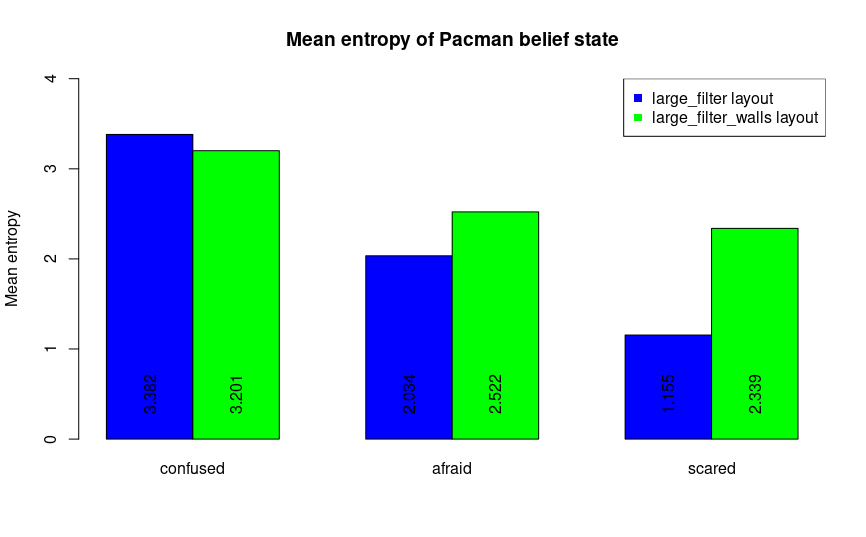
\includegraphics[scale=0.75]{plots/pacman_belief_state.png} 
    \caption{Mean entropy of Pacman's belief state over 10 different runs.}
\end{figure}

\begin{figure}[H]
    \centering
    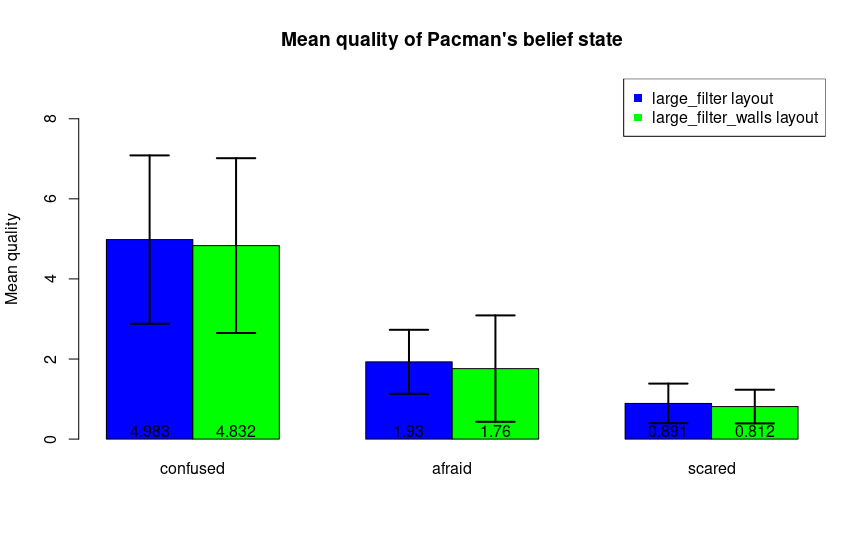
\includegraphics[scale=0.75]{plots/differences.png} 
    \caption{Mean quality of Pacman's belief state over 10 different runs.}
\end{figure}
    
    \item We can see, by using our measures and the model itself, that the values of Pacman's belief state are more concentrated in the maze with the scared and afraid ghosts than with the confused ghost. It is because these ghosts have a higher probability to escape from Pacman than to approach it. Thus, they are reaching a corner of the maze and the measures are more concentrated in the maze : the entropy is lower.
    Moreover, we can see that, for the same reasons, the quality of Pacman's belief state is better with the afraid and scared ghosts than with the confused one. It can seem intuitive that with a more concentrated belief state (lower entropy), the belief state of Pacman is of better quality. In general, in the \texttt{large\_filter} layout, Pacman's belief state has a better entropy and quality than in the \texttt{large\_filter\_walls} because the ghost has a higher probability to go in a corner of the maze : they are less walls preventing it to reach a corner.
    \item Reducing the variance of the sensor will reduce the noise in the distances between the ghosts and Pacman obtained from the sensor. This can be verified in a more mathematical way. We know that the noise is given by: $$\text{noise} = Binom(n, p) - n * p$$
    where $n = \frac{\text{sensor\_variance}}{p^2}$ and $p = 0.5$. Thus, increasing the sensor\_variance will lead to bigger values for the noise. While reducing the sensor\_variance will lead to smaller values for the noise. So, the entropy of Pacman's belief state will be lower with a low sensor\_variance and of better quality.
    
    \item For each remaining ghost, we could only consider the cell which has the highest probability\footnote{If there are multiple cells that have the same highest probability of containing the ghost, we keep the one which is the closest to Pacman.} of containing the ghost. Based on these cells, we compute the least cost path between Pacman and this cell. Then, we play the first move of this path and repeat this process at each iteration : note that when we start to chase one ghost, we will keep chasing it until we ate it in order to save time. This will force Pacman to kill all the ghosts in a minimal number of moves which will increase the score of Pacman at the end of the game.
    \item \textbf{\textit{Leave empty.}}
\end{enumerate}

% ==============================================================================

\end{document}

    \item \textbf{\textit{Leave empty.}}
\end{enumerate}

% ==============================================================================

\end{document}
